\documentclass[final]{article}


\usepackage{APS360}
\usepackage[utf8]{inputenc} % allow utf-8 input
\usepackage[T1]{fontenc}    % use 8-bit T1 fonts
\usepackage{hyperref}       % hyperlinks
\usepackage{url}            % simple URL typesetting
\usepackage{booktabs}       % professional-quality tables
\usepackage{amsfonts}       % blackboard math symbols
\usepackage{nicefrac}       % compact symbols for 1/2, etc.
\usepackage{microtype}      % microtypography
\usepackage{xcolor}         % colors
\usepackage{graphicx}    % image
 
\title{Facial Expression Detection}

\author{%
  Chester Chiow Yong Xun\\
  1012873865, chester.chiow@mail.utoronto.ca\\
  https://github.com/ChesterChiow/FacialExpressionDetection.git\\
}

\begin{document}

\maketitle

\vspace{-0.5in}

\section*{Introduction}
Human facial expressions are one of the most important and universal forms of non-verbal communication. The ability to accurately recognise facial expressions helps us understand one's emotions and decide how to respond appropriately \citep{suslow2023interpersonal}. This is especially crucial in enhancing human-computer interactions systems, where detecting a user's emotional state can help virtual assistants, robots or applications respond better to user's needs. It also has important applications in healthcare such as detecting signs of stress.

The goal of this project is to create and build a deep learning model capable of classifying facial expressions into discrete emotional categories. Deep learning, specifically convolutional neural networks (CNN), will be best suited for image based tasks because it is able to detect important features such as edges, textures, and patterns in facial images. These features are important for distinguishing differences between expressions, making CNN an appropriate tool for accurate facial expression detection.

\section*{Illustration}
The following Figure \ref{fig:sample} shows the overall pipeline and model of the project.

\begin{figure}[!h]
  \centering
  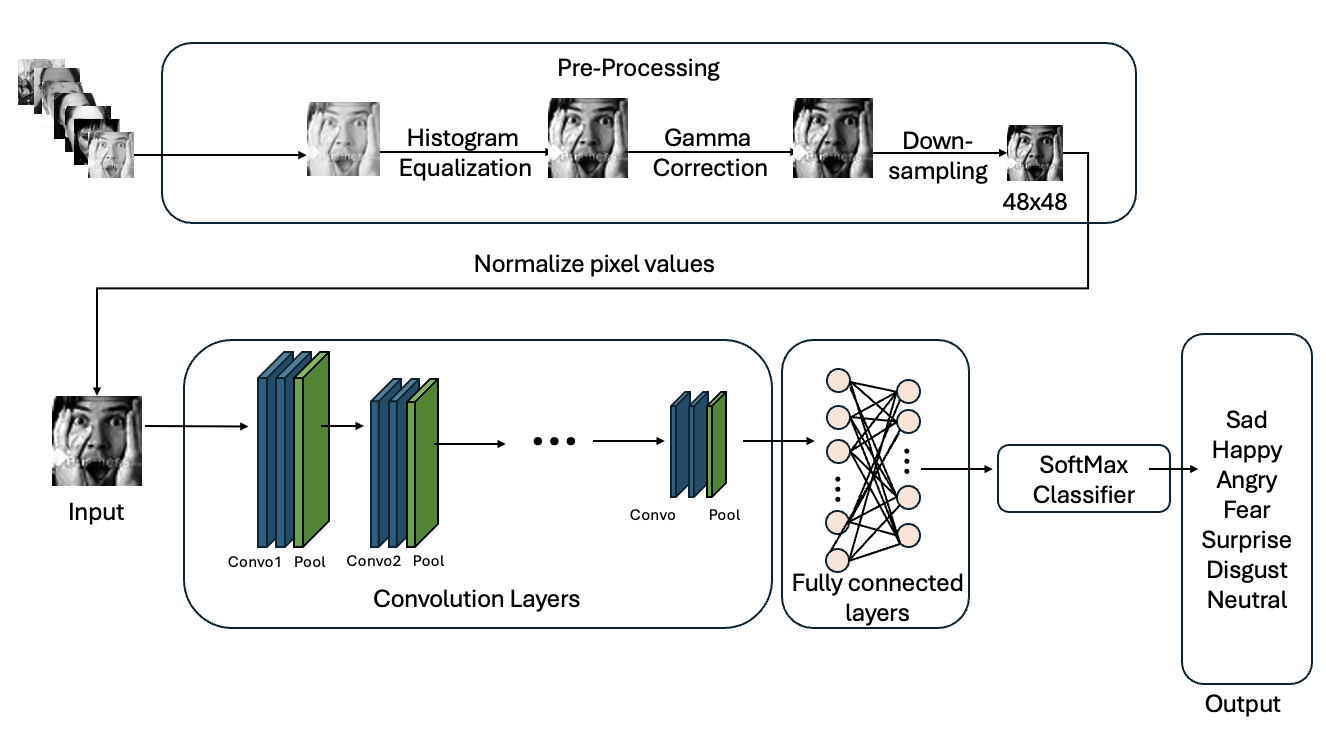
\includegraphics[width=0.6\textwidth]{Proposal_Illustration.png}
  \caption{Facial expression detection model pipeline.}
  \label{fig:sample}
\end{figure}

\section*{Background \& Related Work}
Facial expression detection has been widely studied as it plays an important role in human-computer interaction systems. The Facial Action Coding System (FACS), developed by Ekman and Fiesen in 1978, provides a foundational framework for understanding facial expressions. It categorises facial movements into specific muscle-based action units and is widely used in psychological and human-computer interaction research. Facial expression detection systems reference FACS to classify complex facial behaviours, together with machine learning algorithms \citep{farnsworth2022facs}.

Early research often combined Histogram of Oriented Gradients (HOG) features and support vector machine (SVM) classifiers to detect facial expressions. For example, a study on the application of HOG descriptors in facial expression recognition highlighted its effectiveness in the classification task \citep{carcagni2015hog}. However, more recent studies have shown that CNN algorithms can acheive better performance. A study conducted to compare the effectiveness of CNN and SVM algorithms in classifying human images into stress and non-stress categories showed that CNN outperformed SVM in all evaluation metrics. Its ability to learn complex spatial features from facial images made it well suited for facial expression recognition tasks \citep{royan2025cnnsvm}.

These algorithmic advances have been in implemented in practical tools. One example is OpenFace, an open source toolkit that leverages on facial landmark motion, head pose, facial expression and eye gaze to provide real-time facial behaviour analysis \citep{baltrusaitis2016openface}. Similarly, companies such as Affectiva have developed facial expression recognition solutions like Emotion AI, which combines facial expression detection with other cues, including body language, using deep learning. This enables real-time emotion detection in various industries like healthcare, marketing and automotive \citep{affectiva_emotionAI}.


\section*{Data Processing}
The source dataset used in this project is FER-2013, which consists of 32,398 grayscale facial images \citep{sambare2017fer2013}. To address the low-contrast nature of some images, histogram equalization is applied to enhance local contrast and bring out subtle facial details. Additionally, gamma correction will be used to normalize variations in lighting conditions. Downsampling is then applied to reduce computational load. The preprocessing techniques helps to improve the visibility of key facial features such as the eyes and mouth, which will be important for accurate emotion detection. Finally, all images will be normalized to ensure consistency in pixel intensity distributions.

\section*{Architecture}
This project will use convolutional neural network (CNN) as it is well suited for extracting patterns and features from images. The network will consist of convolutional and pooling layers for feature extraction, batch normalization and dropout to reduce overfitting, fully connected dense layers and softmax output layer with 7 categories (happy, sad, angry, surprise, neutral, disgust, fear).

\section*{Baseline Model}
To establish a reference point, a baseline model will be using a SVM classifier will be implemented. HOG will be used to extract features from the images, as it is able to captures edge and gradient structures. These features are then fed into the SVM, which learns to separate the different emotion classes based on the patterns present in the feature space.

\section*{Ethical Considerations}
The dataset may not fully represent all ethnicities and age groups in expressing emotions. Hence, the dataset may be biased and could lead to inaccurate predictions for underrepresented groups.

Facial expressions may not always accurately reflect one's emotions. Other forms of communication such as verbal cues,  should also be considered to completely understand one's emotional state. For example, a smile does not always mean happiness. Hence, misinterpretation could lead to serious consequences, particularly in sensitive sectors like healthcare and law.


\newpage
\bibliographystyle{apalike} 
\bibliography{refs}


\end{document}